% RESULTADOS-------------------------------------------------------------------

\chapter{Análise e Discussão dos Resultados}
\label{chap:resultados}

Este capítulo discute os resultados obtidos no experimento de detecção de cópias de vídeos através da aplicação das assinaturas digitais revisadas neste trabalho sobre os conjuntos de parametrização e teste detalhados na Seção~\ref{sec:met-Experimentos}.

Conforme detalhado na seção anterior, para a determinação do limiar de classificação de cada assinatura, são realizadas simulações de classificação utilizando um intervalo de limiares. Os casos de parametrização de cada assinatura são dividos em 5 subconjuntos e ao final, é utilizada a média dos limiares resultantes da simulação com cada subconjunto como limiar para a assinatura. Na Figura~\ref{fig:todos-limiares}, foram plotados os valores de precisão, revocação e \textit{fmeasure} para cada assinatura ao longo das simulações com diferentes limiares. O ponto vermelho de cada sub-gráfico ilustra como é feita a escolha de um limiar para cada assinatura.


\begin{figure}[h]
	\centering
	\caption{Exemplo de simulação de classificação para cada um dos tipos de assinatura. O eixo X é composto dos limiares testados para a assinatura. Os pontos vermelhos indicam o valor máximo de \textit{fmeasure}, ponto em que o limiar apresenta o melhor resultado.}
	\label{fig:todos-limiares}
	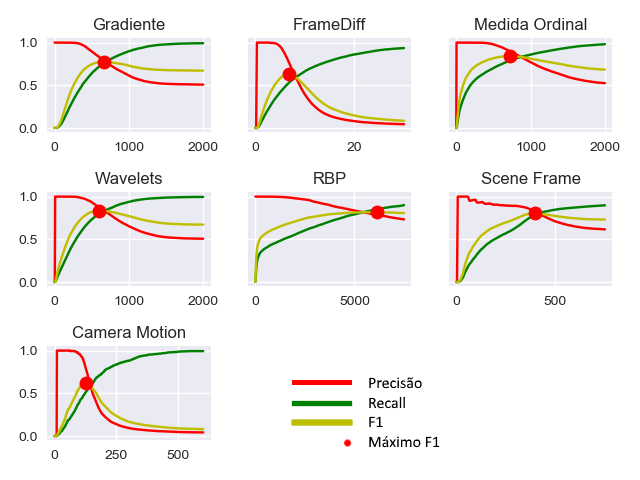
\includegraphics[width=\textwidth]{dados/figuras/experimentos/todos_final.png}
\end{figure}

Os subconjuntos de parametrização foram nomeados de T.1 a T.5 e o melhor limiar resultante da simulação com cada subconjunto está disposto na Tabela~\ref{tab:limiares}, além do limiar final de cada algoritmo.

\begin{table}[h]
	\caption{Limiares obtidos nas simulações com cada subconjunto de parametrização.}
	\label{tab:limiares}
	\begin{tabular}{|l|r|r|r|r|r|r|}
		\hline
		\textbf{Assinatura} & \textbf{T.1} & \textbf{T.2} & \textbf{T.3} & \textbf{T.4} & \textbf{T.5} & \textbf{Limiar Final}\\ \hline
		Gradiente & 761.52 & 637.27 & 681.36 & 705.41 & 629.25 & 682.96\\ \hline
		FrameDiff & 6.63 & 6.48 & 6.33 & 6.78 & 6.93 & 6.63\\ \hline
		Medida Ordinal & 657.31 & 729.45 & 661.32 & 725.45 & 749.49 & 704.60\\ \hline
		Wavelets & 597.19 & 593.18 & 625.25 & 601.20 & 625.25 & 608.41\\ \hline
		RBP & 5501.00 & 6793.58 & 6553.10 & 6147.29 & 4569.13 & 5912.82\\ \hline
		Scene Frame & 399.49 & 391.95 & 399.49 & 391.95 & 399.49 & 396.48\\ \hline
		Camera Motion & 111.82 & 123.84 & 107.01 & 139.47 & 128.65 & 122.16\\ \hline
	\end{tabular}
\end{table}

Na sequência, serão discutidos os resultados obtidos nos testes utilizando os limiares definidos na etapa anterior para cada tipo de assinatura. As assinaturas serão analisadas quanto a sua robustez e unicidade por tipo de distorção aplicada (fotométrica, geométrica ou temporal). Por fim, será avaliado se a junção de um algoritmo temporal (camera motion) e um algoritmo espacial é mais eficaz em detectar cópias de vídeo que a utilização de um tipo de assinatura de forma isolada. 

\section{Robustez}

Segundo \citeauthor{hua2004robust}, robustez é a capacidade de uma assinatura ser tolerante a ruído, o que quer dizer que dois vídeos com o mesmo conteúdo devem ter assinaturas idênticas ou muito similares, mesmo que eles tenham passado por algum tipo de distorção. Esta é uma das duas propriedades desejadas em uma assinatura, a outra sendo unicidade, que será abordada na próxima seção.

Ao tentar determinar a robustez de um algoritmo, leva-se em consideração apenas os casos de teste em que de fato um par de vídeos tem o mesmo conteúdo, ou seja, o vídeo de teste é uma cópia do vídeo original. A partir daí, a pergunta levantada é "quantos destes casos de cópia a assinatura consegue classificar corretamente?", ou em termos de recuperação de informações "quantos elementos relevantes foram selecionados?". Esta é exatamente a definição da medida de revocação~\cite{Ting2010}, que foi utilizada para este teste. As medidas de revocação obtidas para cada assinaturas podem ser vistas na Figura~\ref{fig:heatmap-revocacao}.


\begin{figure}[h]
	\centering
	\caption{Mapa de calor de revocação de cada tipo de assinatura com cada tipo de distorção}
	\label{fig:heatmap-revocacao}
	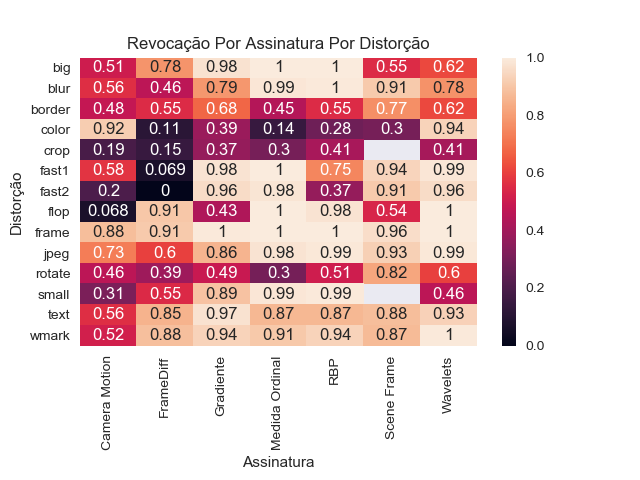
\includegraphics[width=\textwidth]{dados/figuras/experimentos/heatmap_final_recall.png}	
\end{figure}

As assinaturas temporais (Camera Motion e FrameDiff) obtiveram os piores resultados na análise da robustez em geral, sendo que elas são especialmente afetadas pelas distorções temporais de aceleração fast1 e fast2. É possível notar também que a medida com que os vídeos foram mais acelerados, as assinaturas temporais tiveram resultados piores. A assinatura temporal FrameDiff obteve aproximadamente 6\% no teste com a distorção fast1 e e 0\% com a distorção fast2, mostrando que esse tipo de assinatura é extremamente sensível à perda de informação causada pela diminuição do número de quadros de um vídeo. A Camera Motion foi mais sensível a distorção flop, que inverte o vídeo horizontalmente. Isso faz sentido pois esta distorção inverte a translação e rotação da câmera. A última distorção temporal, frame, foi a que causou menos problemas para as assinaturas em geral (3 delas conseguiram classificar corretamente em 100\% dos casos e todas as outras têm revocação maior que 80\%), pois a quantidade de quadros retirados de um vídeo é pequena se comparado às outras distorções temporais, além disso este tipo de distorção é pouco perceptível por humanos.

Outras distorções que tiveram pouco efeito sobre a classificação são as que adicionam textos de forma uniforme nos vídeos: text e wmark. O único caso em que estas distorções afetaram significativamente a classificação é com a utilização da assinatura Camera Motion. Como ela se baseia no rastreamento do movimento de regiões do vídeo entre os quadros, o posicionamento estático do texto realizado pela distorção o impede de acompanhar os movimentos precisamente.

Entre as distorções fotométricas, a color foi a mais efetiva em enganar a detecção de cópias, apenas as assinaturas Camera Motion e Wavelets conseguiram resultados bom com revocação acima dos 90\%, enquanto todas as outras assinaturas obteram valores de revocação abaixo de 40\%. Os resultados favoráveis a essas duas assinaturas se devem ao fato destas não utilizarem valores de luminância para descrever um vídeo, enquanto os outros o fazem. Já a distorção blur afetou negativamente todos as assinaturas que usam bordas ou pequenas regiões de interesse para descrever um vídeo, pois enfraquece os detalhes de um quadro. A distorção jpeg teve resultados semelhantes por também causar uma perda de informação dentro de cada quadro do vídeo. 

% Por fim, as assinaturas geométricas...
% No geral, a assinatura... para fotométricas, para temporais e geométricas

A revocação sozinha não pode ser utilizada para a avaliação de uma assinatura, pois bastaria marcar todos os pares de vídeos como sendo cópias para atingir um valor de 100\% de revocação. Vê-se necessária uma análise complementar à da robustez, sobre a capacidade discriminante de uma assinatura: a unicidade. A seção a seguir discute sua definição, apresenta uma forma de medi-la e avalia cada assinatura quanto a essa métrica.

% Verificar se consegue encontrar a cópia
\section{Unicidade}

Segundo \citeauthor{hua2004robust}, unicidade é a capacidade discriminativa de uma assinatura de vídeo, o que significa que vídeos com conteúdos diferentes devem ter assinaturas diferentes. Esta característica é essencial para a utilidade de uma assinatura, pois uma técnica que gera muitos casos de falsos positivos perde sua utilidade como ferramenta de automação de detecção de cópias. Para avaliar esta característica, é utilizada a medida de precisão, que mede a quantidade de casos que são relevantes (verdadeiros positivos), dentro de todos os pares de vídeos que são classificados como cópias (verdadeiros positivos e falsos positivos)\cite{Ting2010}.

A Figura~\ref{fig:heatmap-precisao} apresenta os valores de precisão resultados dos testes com todas as assinaturas. Ao comparar estes resultados com os valores da Figura~\ref{fig:heatmap-revocacao}, nota-se uma relação entre as duas: os pontos escuros (piores resultados) e os claros (melhores resultados) estão localizados nas mesmas regiões. No entanto, a diferença de intensidade entre cada assinatura não é proporcional. A Figura~\ref{fig:todos-limiares} apresentada no início deste capítulo mostra a diminuição da capacidade discriminativa de cada assinatura a medida com que o limiar de corte se afasta do zero, além disso, nota-se também que cada assinatura apresenta uma proporção diferente para essa diminuição. As assinaturas Medida Ordinal, Wavelets, Scene Frame e RBP são os que mantém a precisão em níveis mais altos, e isso é refletido na Figura~\ref{fig:heatmap-precisao}.

\begin{figure}[h]
	\centering
	\caption{Mapa de calor de precisão de cada tipo de assinatura com cada tipo de distorção}
	\label{fig:heatmap-precisao}
	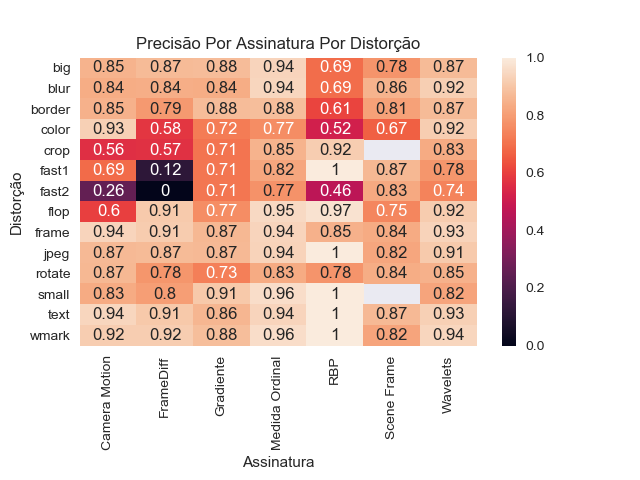
\includegraphics[width=\textwidth]{dados/figuras/experimentos/heatmap_final_precisao.png}	
\end{figure}

Em termos gerais, a assinatura Medida Ordinal tem os melhores resultados neste teste, não apresentando nenhum valor de precisão abaixo de 75\% e tendo valores acima de 90\% para 8 das 14 distorções. Assim como no análise da robustez, as assinaturas temporais obtiveram os piores resultados e o fizeram exatamente nos mesmos casos: fast1, fast2 e flop. Para entender o motivo destes resultados para as assinaturas temporais, foram plotados histogramas dos resultados das comparações de cada assinatura. As séries verdes representam pares de vídeos que são cópias entre si, enquanto que as séries azuis representam não-cópias. A Figura~\ref{fig:histograma-camera-motion} mostra que a assinatura Camera Motion é capaz de distinguir entre a maioria das distorções (embora que não perfeitamente), mas falha quase completamente nas distorções temporais de aceleração (fast1 e fast2) e de inversão de cores(color). Usando este histograma, pode-se afirmar que a escolha do limiar para essa assinatura tem pouco efeito no resultado da sua classificação para essas distorções, pois os grupos de "cópias" e "não-cópias" estão quase completamente sobrepostos e não há como separá-los. O mesmo fenômeno com as distorções temporais pode ser observado na Figura~\ref{fig:histograma-framediff} para a assinatura FrameDiff. 

\begin{figure}[h]
	\centering
	\caption{Histograma de valores resultantes da comparação entre pares de vídeos de teste e vídeos originais para a assinatura Camera Motion. Os casos que são cópias estão marcados de verde, enquanto que os não-cópias estão marcados de azul. Quanto mais afastados os dois grupos, maior o poder de discriminação de cada da assinatura para aquela distorção. Ex: Distorção color}
	\label{fig:histograma-camera-motion}
	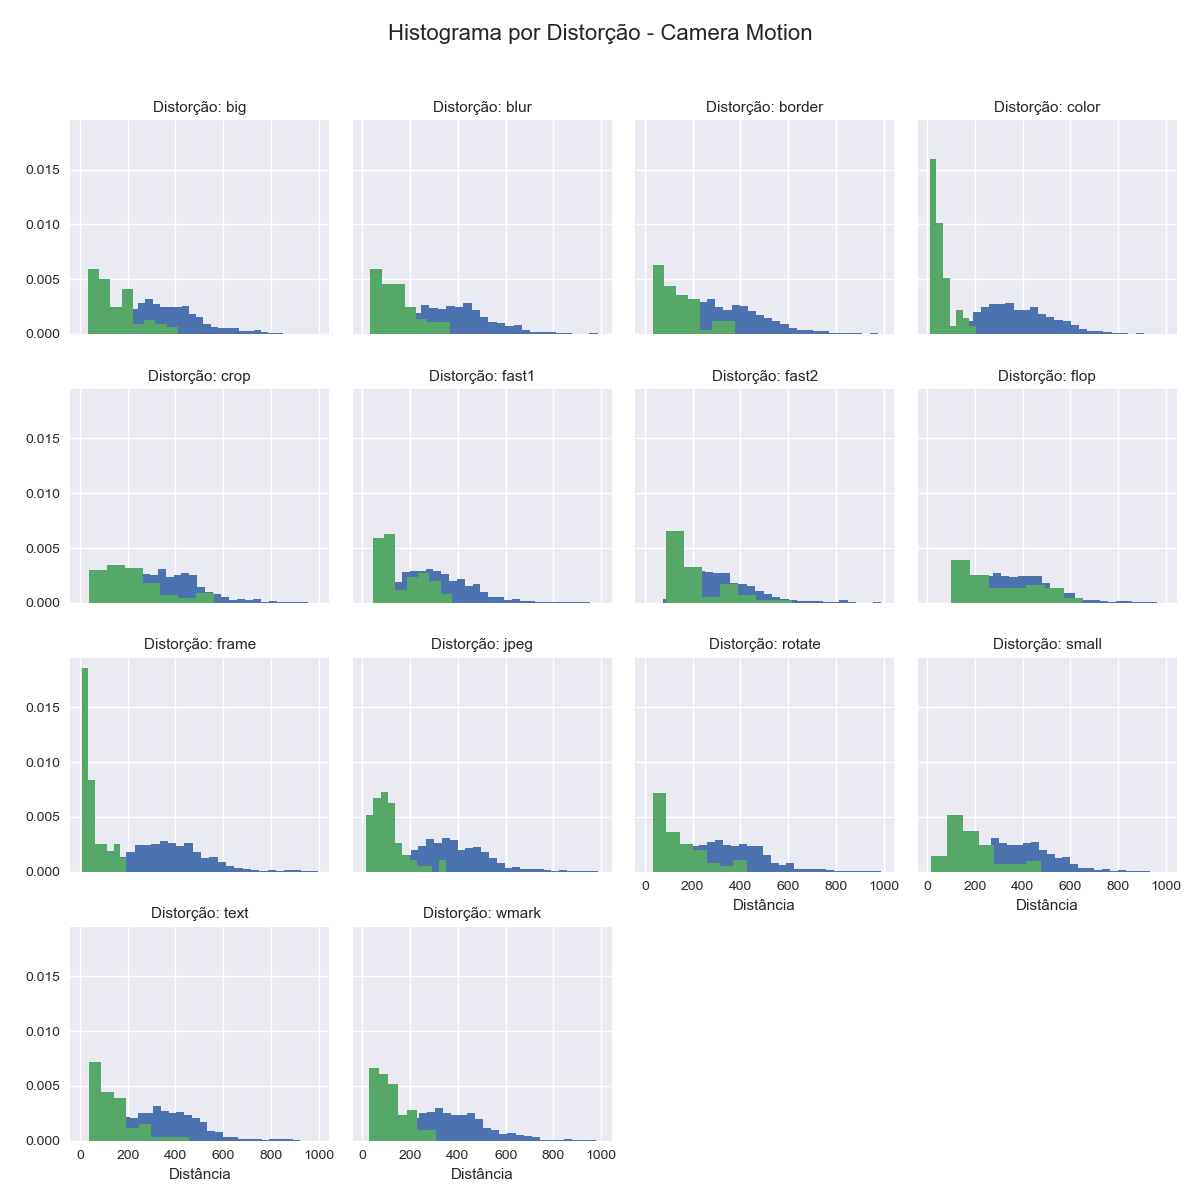
\includegraphics[width=\textwidth]{dados/figuras/experimentos/histograma_distorcao_Camera_Motion.png}
\end{figure}

\begin{figure}[h]
	\centering
	\caption{Histograma de valores resultantes da comparação entre pares de vídeos de teste e vídeos originais para a assinatura FrameDiff. Os casos que são cópias estão marcados de verde, enquanto que os não-cópias estão marcados de azul. Quanto mais afastados os dois grupos, maior o poder de discriminação de cada da assinatura para aquela distorção. Ex: Distorção flop}
	\label{fig:histograma-framediff}
	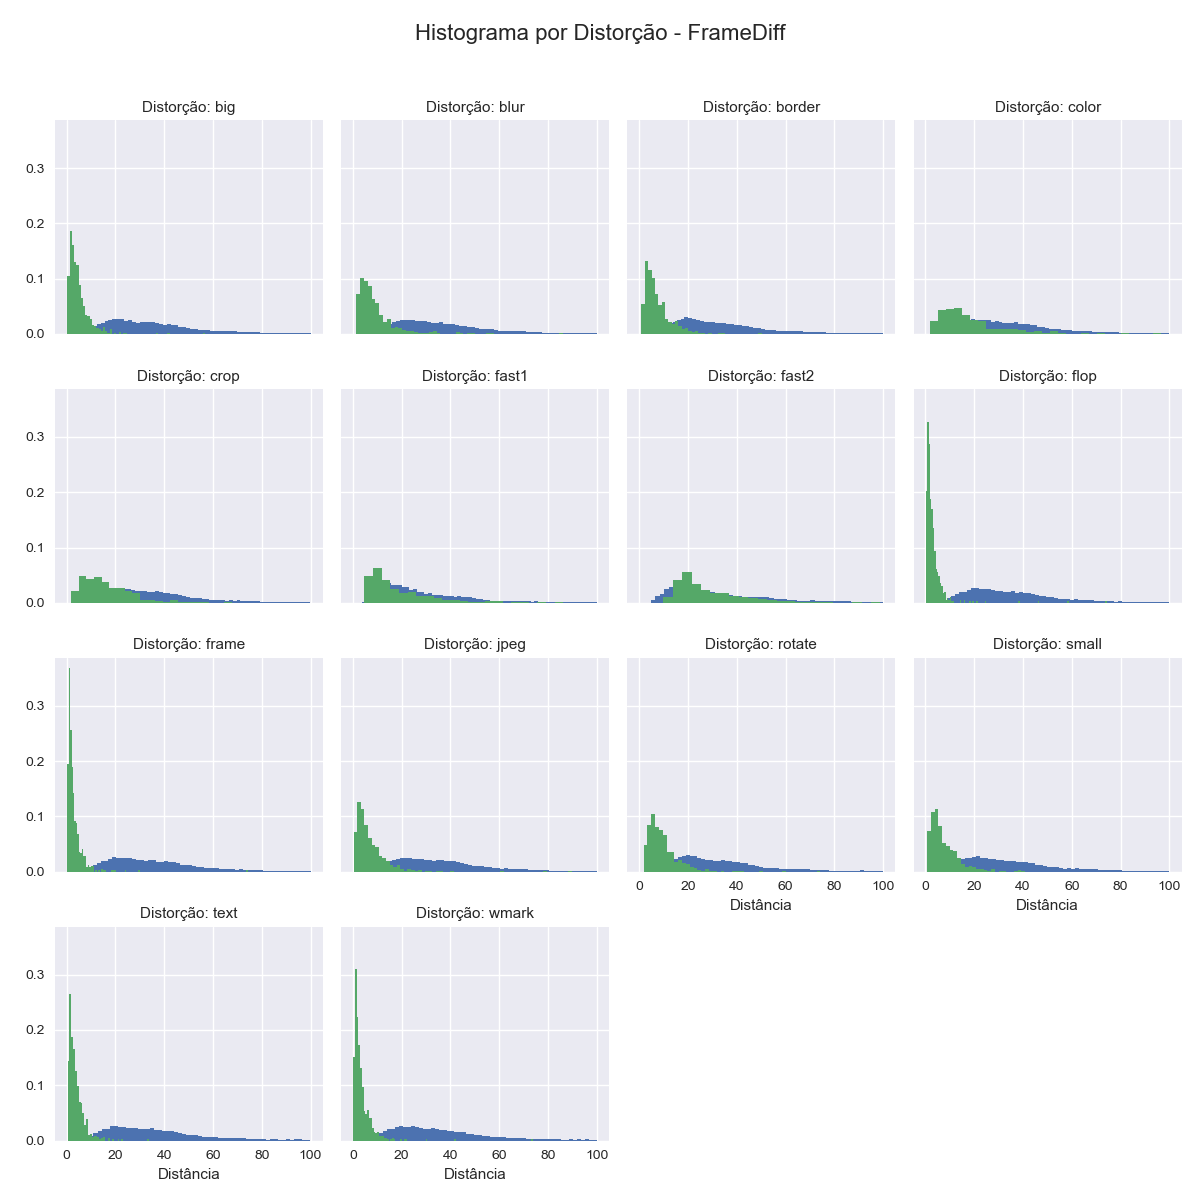
\includegraphics[width=\textwidth]{dados/figuras/experimentos/histograma_distorcao_FrameDiff.png}
\end{figure}

Por fim, para avaliar todas as assinaturas de modo geral, é preciso levar em consideração sua robustez e unicidade simultaneamente. 

\begin{figure}[h]
	\centering
	\caption{Mapa de calor de \textit{fmeasure} de cada tipo de assinatura com cada tipo de distorção}
	\label{fig:heatmap-final_f1}
	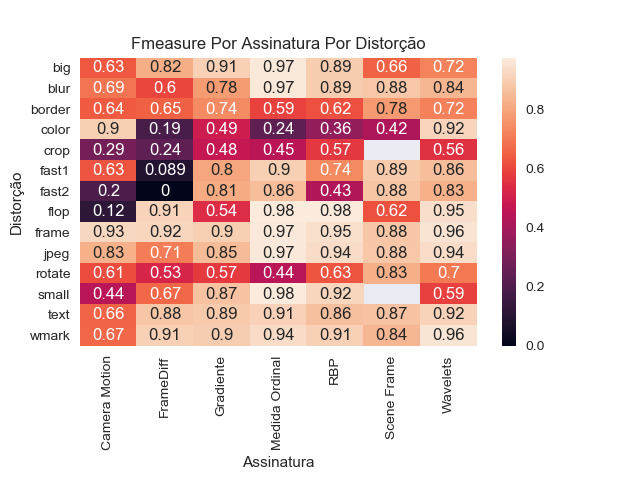
\includegraphics[width=\textwidth]{dados/figuras/experimentos/heatmap_final_f1.png}
\end{figure}

% Verificar se identifica que é cópia de apenas 1 vídeo

% Separar por distorções e discutir o resultado de cada algoritmo
% Mostrar que 

% ------------------------- Treinamento
% \begin{figure}[h]
% 	\centering
% 	\label{fig:limiares-framediff}
% 	\caption{Teste de limiares para a assinatura framediff}
% 	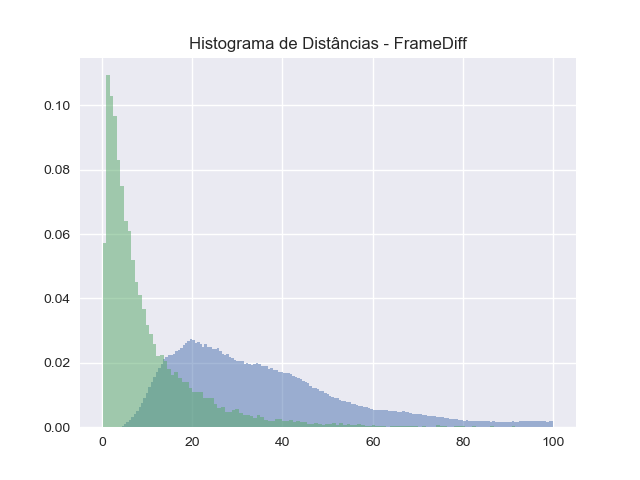
\includegraphics[width=0.8\textwidth]{dados/figuras/experimentos/histograma_FrameDiff.png}
% \end{figure}
% \begin{figure}[h]
% 	\centering
% 	\label{fig:limiares-medidaordinal}
% 	\caption{Teste de limiares para a assinatura medida ordinal}
% 	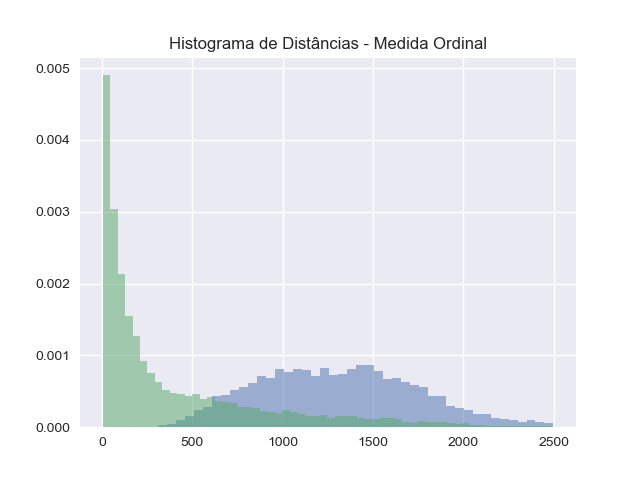
\includegraphics[width=0.8\textwidth]{dados/figuras/experimentos/histograma_Medida_Ordinal.png}
% \end{figure}
% \begin{figure}[h]
% 	\centering
% 	\label{fig:limiares-sceneframe}
% 	\caption{Teste de limiares para a assinatura sceneframe}
% 	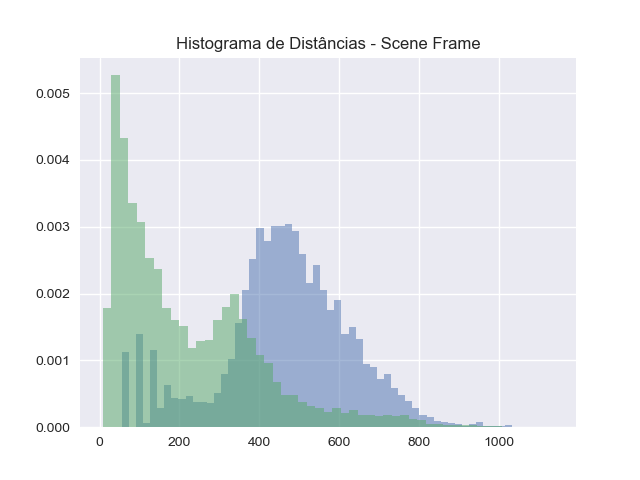
\includegraphics[width=0.8\textwidth]{dados/figuras/experimentos/histograma_Scene_Frame.png}
% \end{figure}
% \begin{figure}[h]
% 	\centering
% 	\label{fig:limiares-gradiente}
% 	\caption{Teste de limiares para a assinatura gradiente}
% 	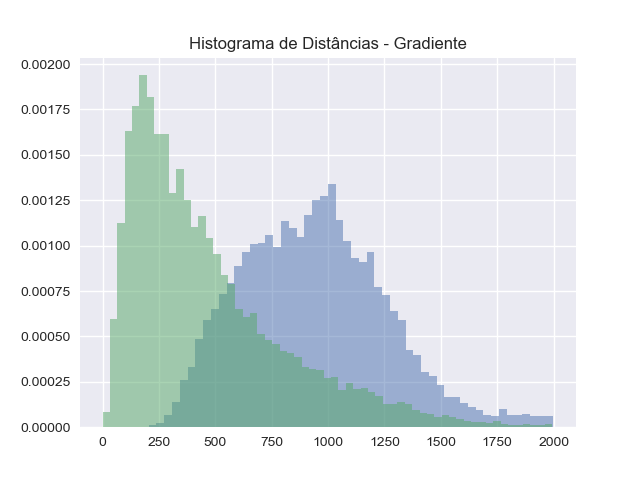
\includegraphics[width=0.8\textwidth]{dados/figuras/experimentos/histograma_Gradiente.png}
% \end{figure}
% \begin{figure}[h]
% 	\centering
% 	\label{fig:limiares-rbp}
% 	\caption{Teste de limiares para a assinatura rbp}
% 	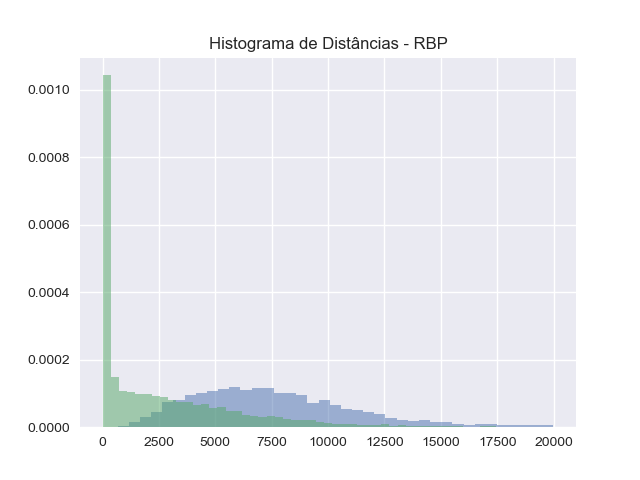
\includegraphics[width=0.8\textwidth]{dados/figuras/experimentos/histograma_RBP.png}
% \end{figure}
% \begin{figure}[h]
% 	\centering
% 	\label{fig:limiares-wavelets}
% 	\caption{Teste de limiares para a assinatura wavelets}
% 	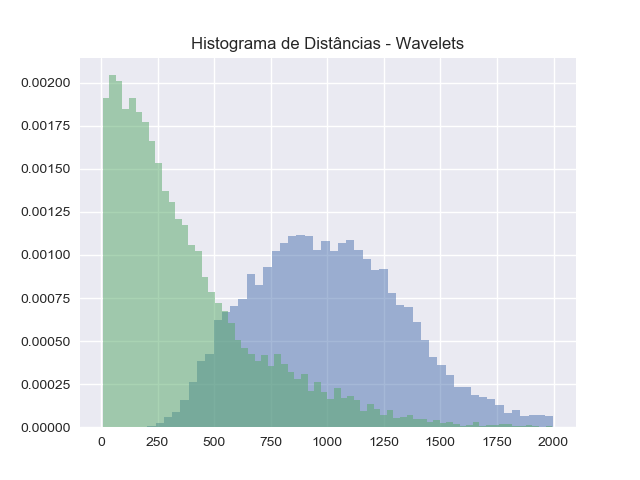
\includegraphics[width=0.8\textwidth]{dados/figuras/experimentos/histograma_Wavelets.png}
% \end{figure}

% \begin{figure}[h]
% 	\centering
% 	\label{fig:limiares-camera-motion}
% 	\caption{Teste de limiares para a assinatura camera motion}
% 	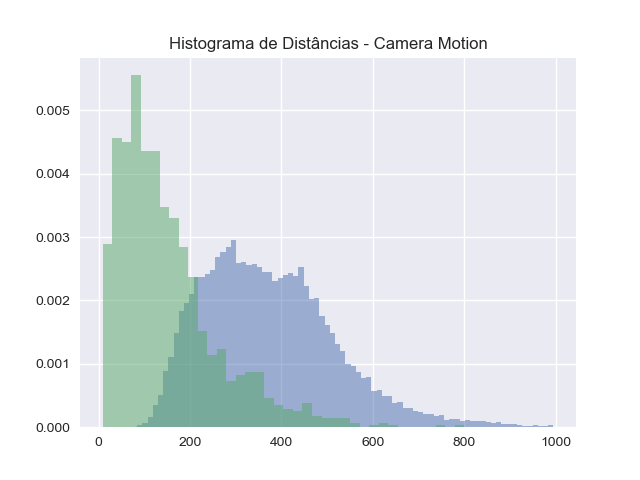
\includegraphics[width=0.8\textwidth]{dados/figuras/experimentos/histograma_Camera_Motion.png}
% \end{figure}

% \begin{figure}[h]
% 	\centering
% 	\label{fig:limiares}
% 	\caption{Limiares}
% 	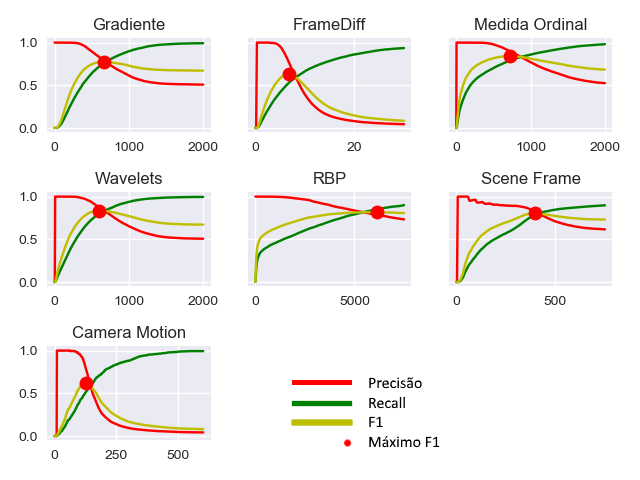
\includegraphics[width=\textwidth]{dados/figuras/experimentos/todos_final.png}
% \end{figure}

% \begin{figure}[h]
% 	\centering
% 	\label{fig:final_heatmap}
% 	\caption{Final}
% 	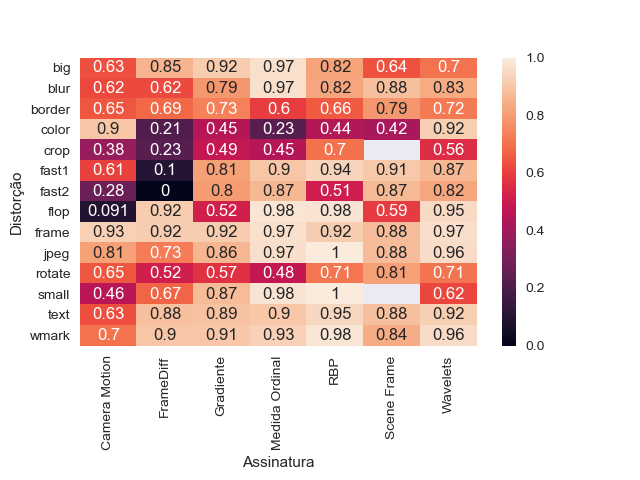
\includegraphics[width=\textwidth]{dados/figuras/experimentos/heatmap_final.png}
% \end{figure}


% \begin{figure}[h]
% 	\centering
% 	\label{fig:limiares-framediff}
% 	\caption{Teste de limiares para a assinatura framediff}
% 	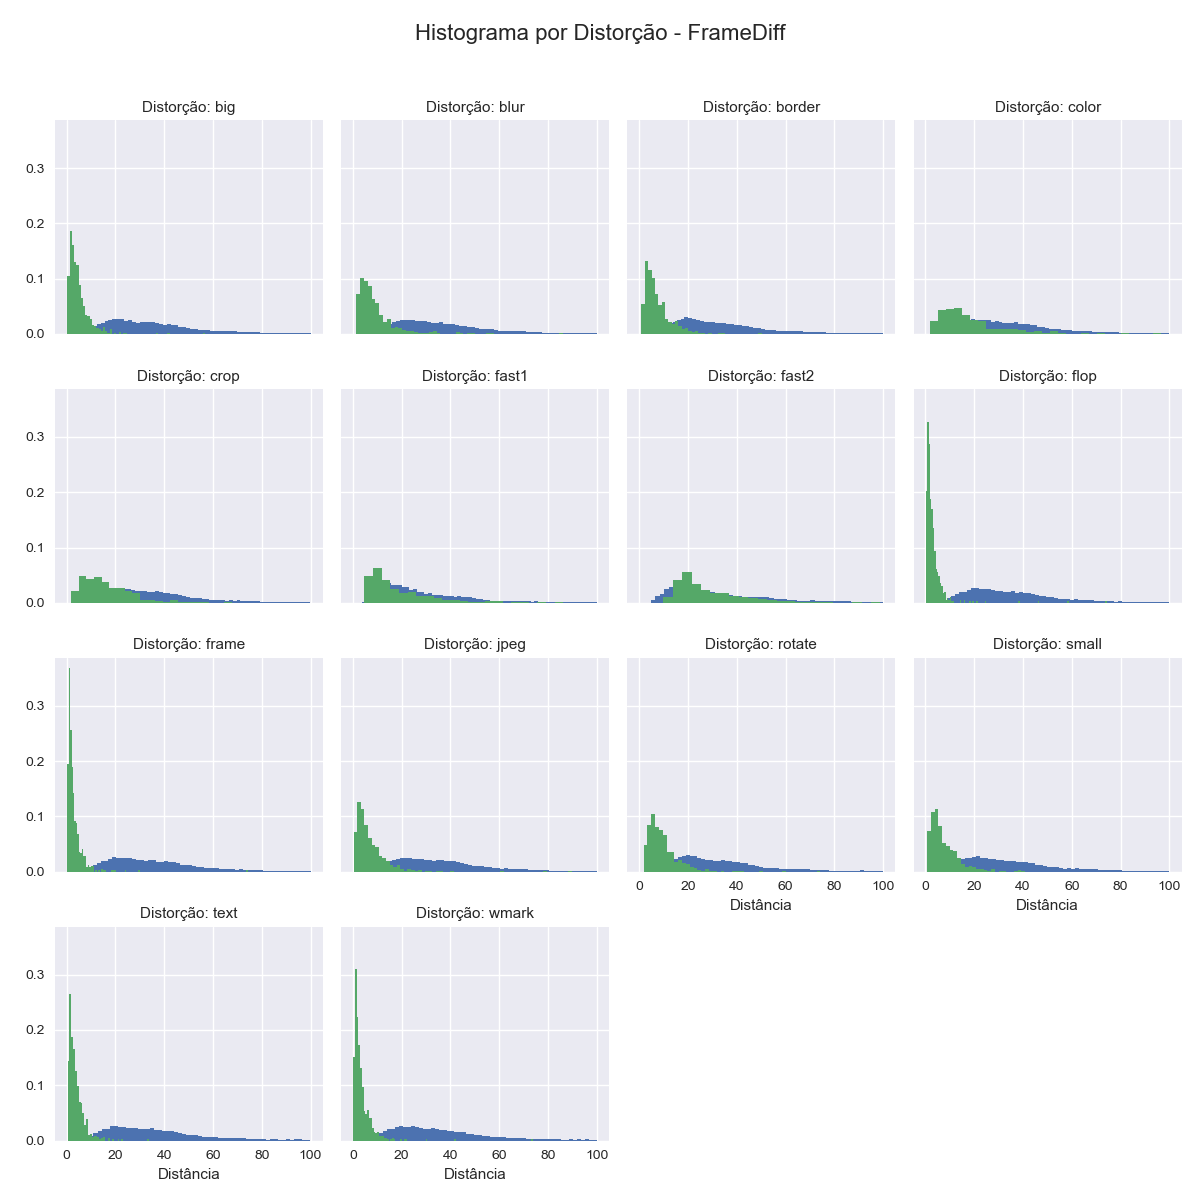
\includegraphics[width=\textwidth]{dados/figuras/experimentos/histograma_distorcao_FrameDiff.png}
% \end{figure}
% \begin{figure}[h]
% 	\centering
% 	\label{fig:limiares-medidaordinal}
% 	\caption{Teste de limiares para a assinatura medida ordinal}
% 	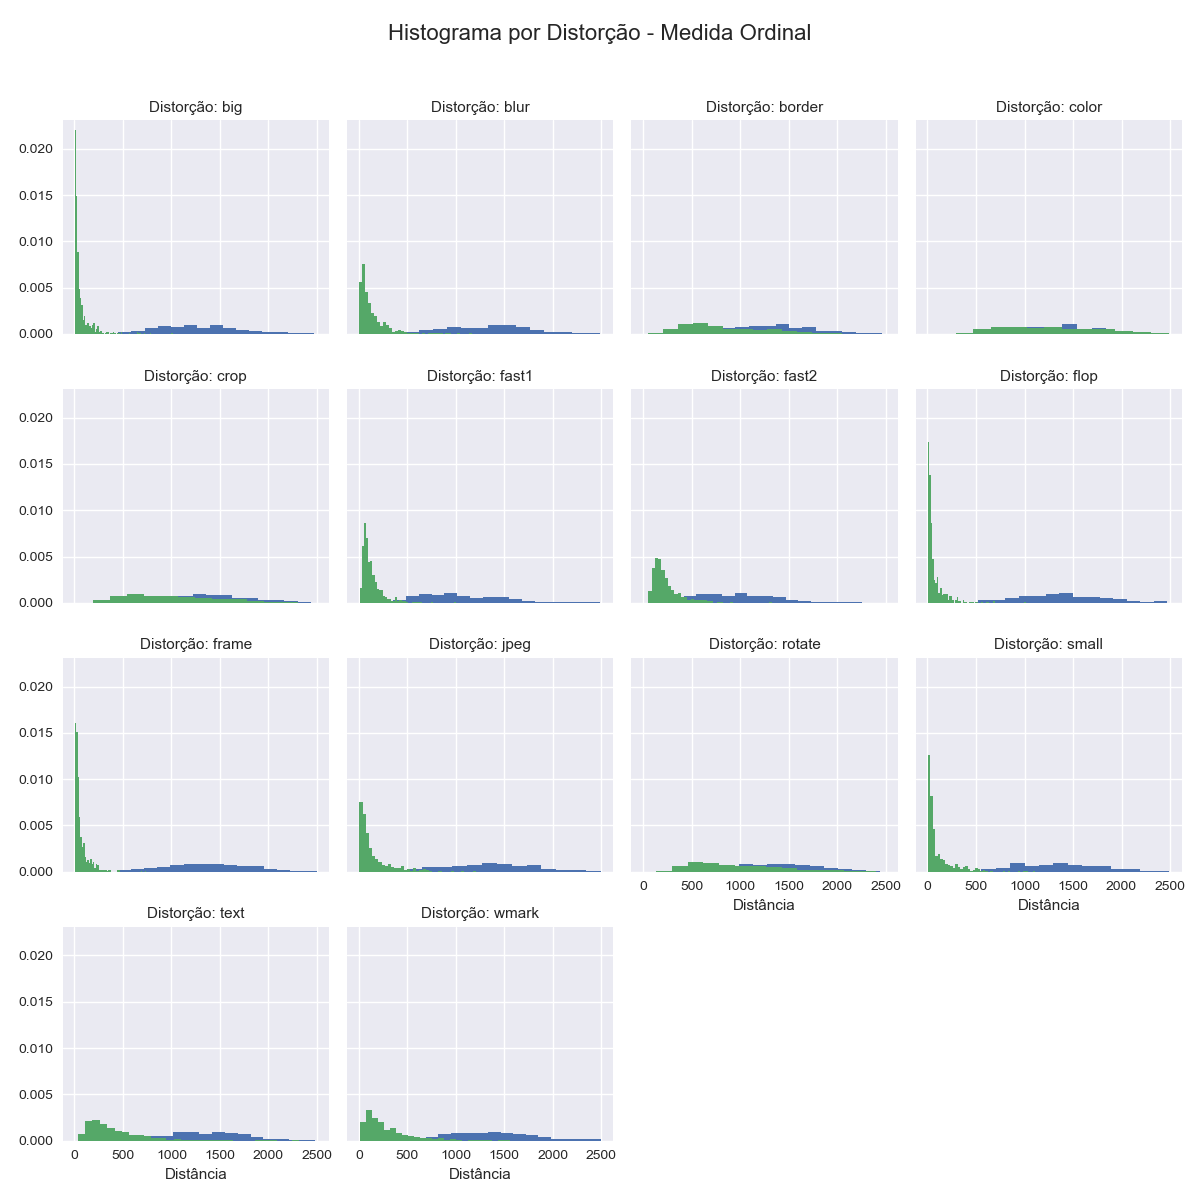
\includegraphics[width=\textwidth]{dados/figuras/experimentos/histograma_distorcao_Medida_Ordinal.png}
% \end{figure}
% \begin{figure}[h]
% 	\centering
% 	\label{fig:limiares-sceneframe}
% 	\caption{Teste de limiares para a assinatura sceneframe}
% 	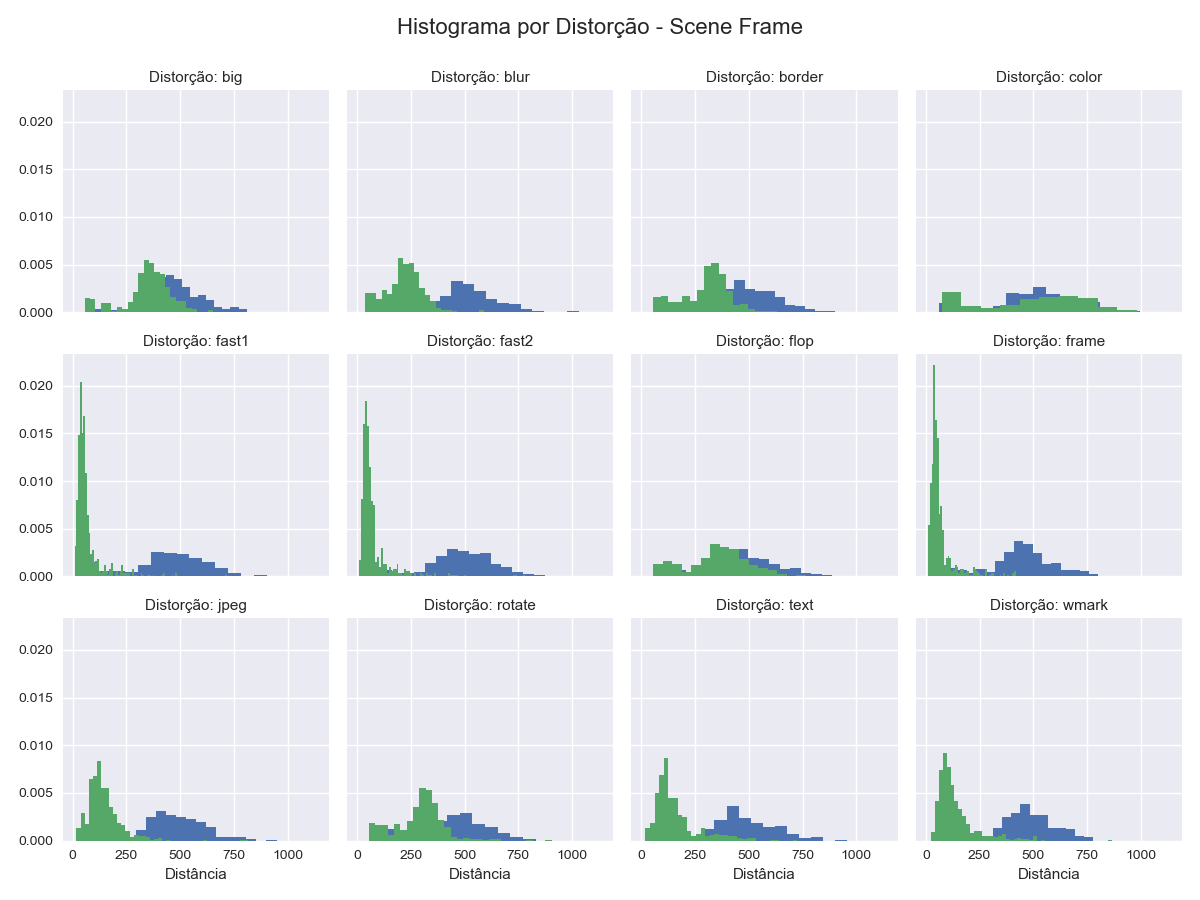
\includegraphics[width=\textwidth]{dados/figuras/experimentos/histograma_distorcao_Scene_Frame.png}
% \end{figure}
% \begin{figure}[h]
% 	\centering
% 	\label{fig:limiares-gradiente}
% 	\caption{Teste de limiares para a assinatura gradiente}
% 	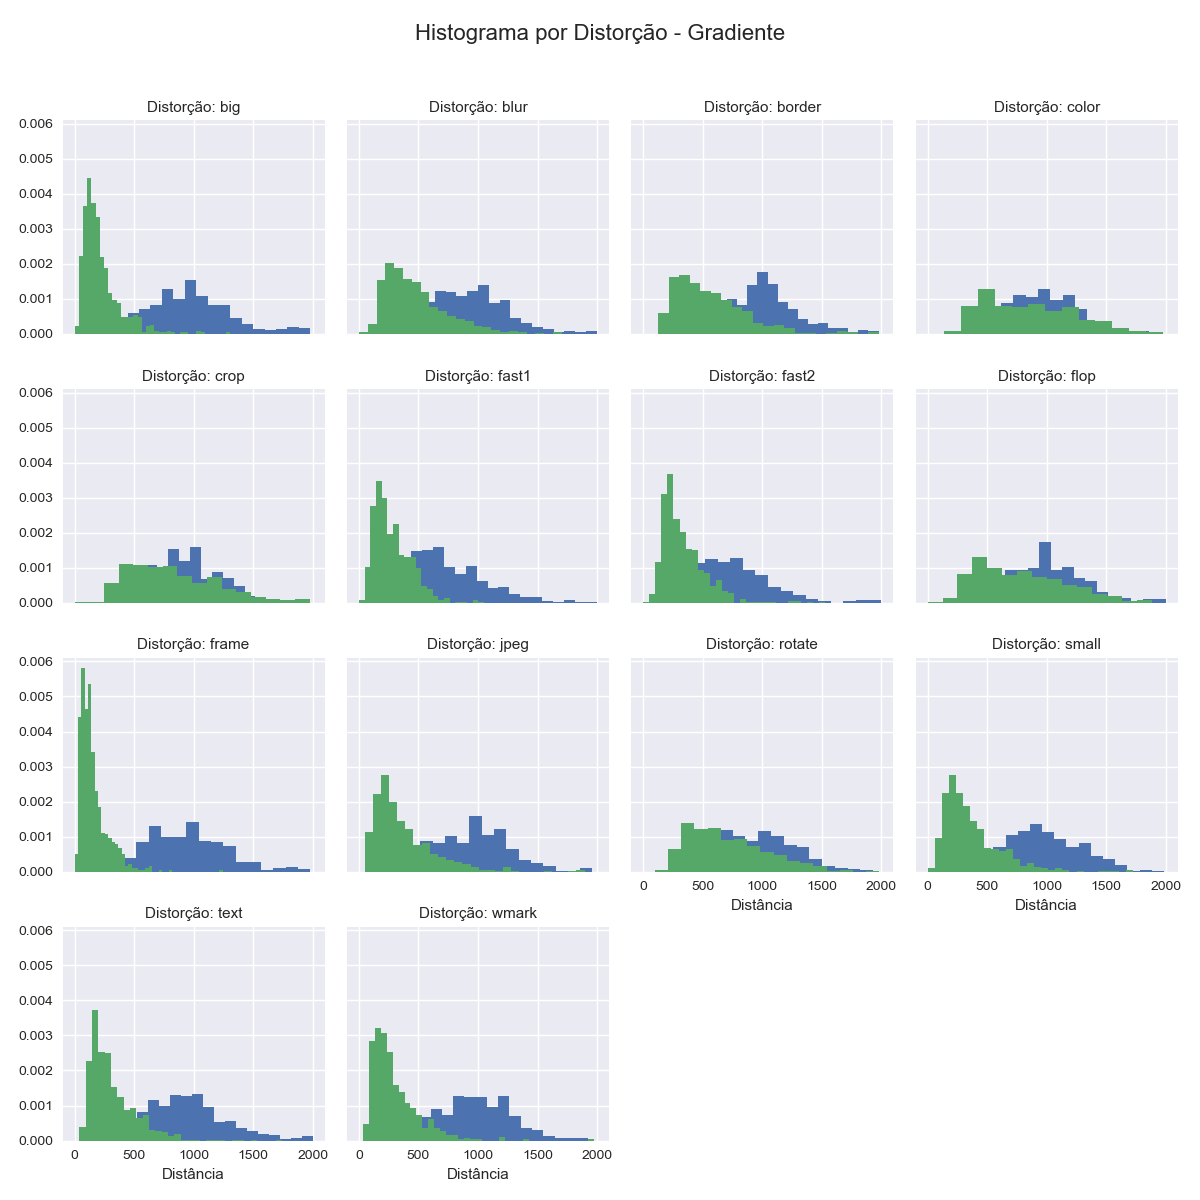
\includegraphics[width=\textwidth]{dados/figuras/experimentos/histograma_distorcao_Gradiente.png}
% \end{figure}
% \begin{figure}[h]
% 	\centering
% 	\label{fig:limiares-rbp}
% 	\caption{Teste de limiares para a assinatura rbp}
% 	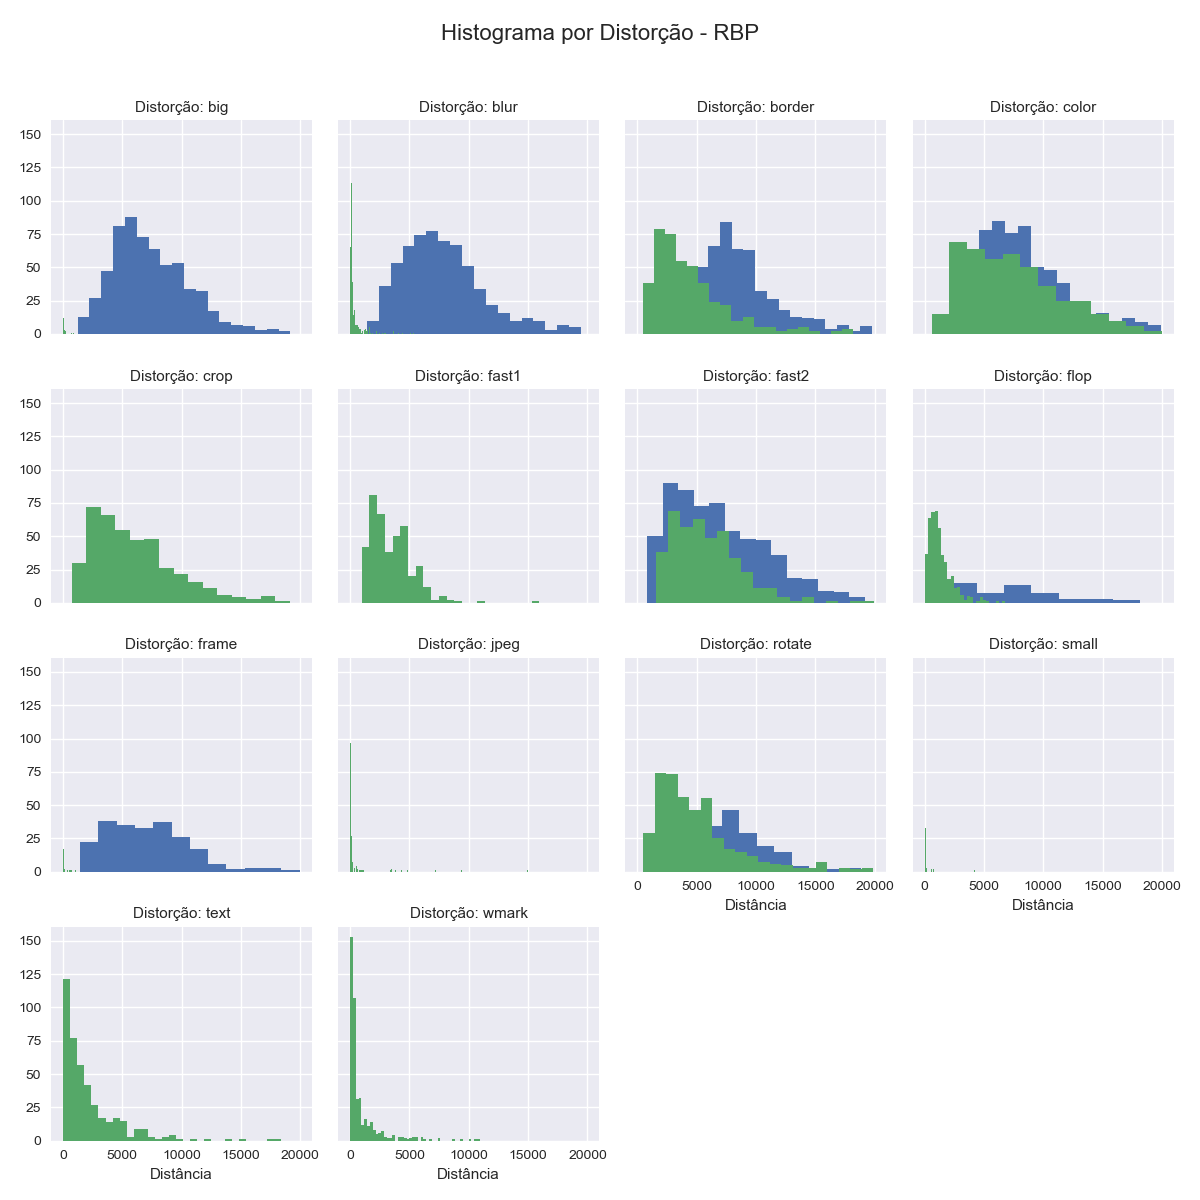
\includegraphics[width=\textwidth]{dados/figuras/experimentos/histograma_distorcao_RBP.png}
% \end{figure}
% \begin{figure}[h]
% 	\centering
% 	\label{fig:limiares-wavelets}
% 	\caption{Teste de limiares para a assinatura wavelets}
% 	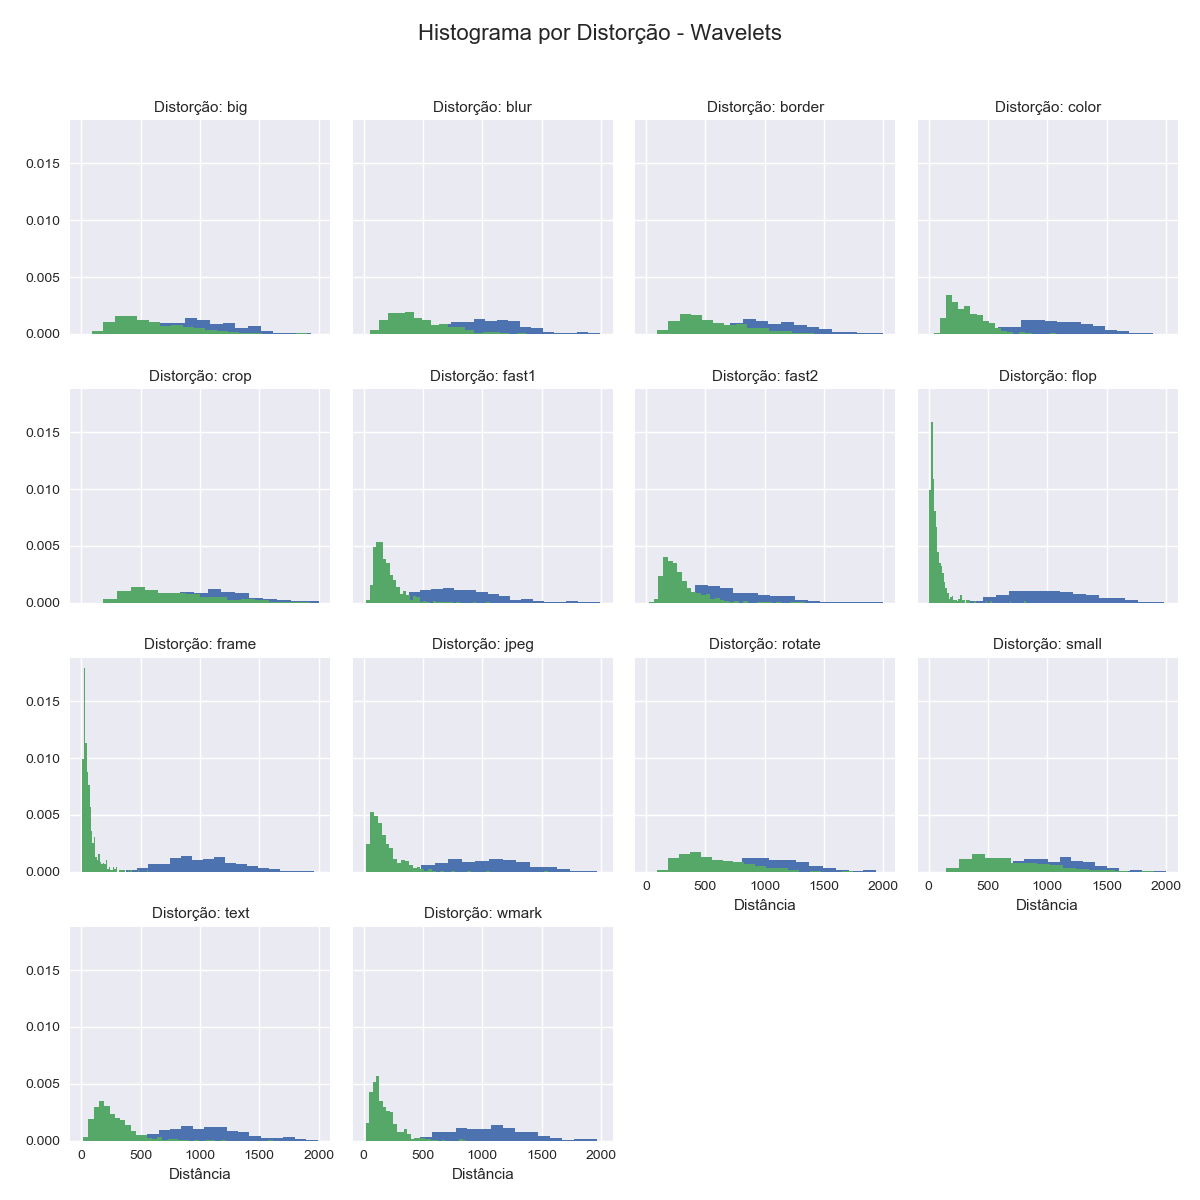
\includegraphics[width=\textwidth]{dados/figuras/experimentos/histograma_distorcao_Wavelets.png}
% \end{figure}

% \begin{figure}[h]
% 	\centering
% 	\label{fig:limiares-camera-motion}
% 	\caption{Teste de limiares para a assinatura camera motion}
% 	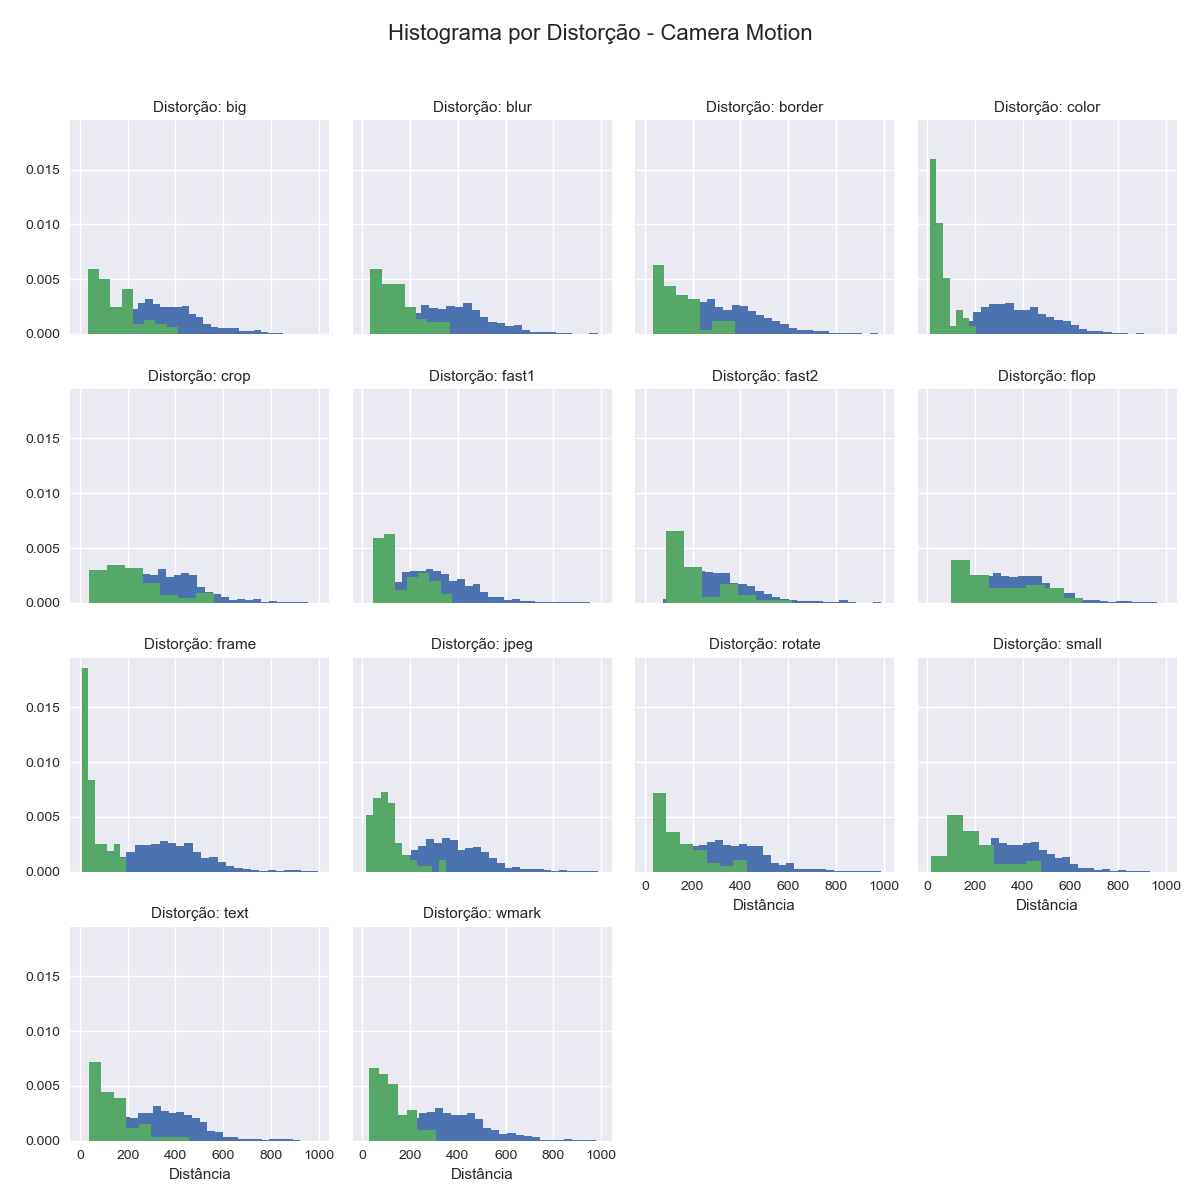
\includegraphics[width=\textwidth]{dados/figuras/experimentos/histograma_distorcao_Camera_Motion.png}
% \end{figure}
